% In Figures~\ref{fig:impl0:20miccross} and \ref{fig:impl0:5miccross}, we saw that, at very low scan speeds, the control signal shows lots of oscillation. These are caused by building vibration electrical noise and are amplified by the $z$-axis control loop.
\section{Improving the $Z$-axis}\label{chap:zaxis-improv}

In this chapter, we improve the $Z$-axis control. The chapter is broken into two main sections. First, we study unwanted external disturbances imposing themselves on the $Z$-axis dynamics, their implications for control, and methods to mitigate them. In the second section, we design a relatively simple control scheme. The twist is that we enable automated identification and design.

\section{$Z$-axis disturbances}\label{sec:zaxis-dist}
First, we study how external disturbances enter the $Z$-axis control loop. We then show that, given a set of disturbances within some frequency band, we must limit the control bandwidth, and consequently the imaging speed, or resign ourselves to having the disturbances show up in our images. We then study the specific disturbances present in our experimental setup. Finally, we identify the source of two specific disturbances and show how they can be mitigated inexpensively.

\subsection{General Implications of Disturbances}

Figure \ref{fig:zimprv:z_axis_bd} shows a block diagram of the $z$-axis control loop.
The two relevant transfer functions are
\begin{align}
  H_{ed} &= \frac{-1}{1 + GD}\\
  H_{ud} &= \frac{-D}{1 + GD}, \label{eqn:hud}
\end{align}
which are the transfer function from the disturbance to the error and from the disturbance to the control. Here, $d=s+d_{\text{ext}}$, where $s(t)$ is the sample surface and $d_{\text{ext}}(t)$ is an external disturbance. Typically, the cantilever dynamics are much faster than the rest of the control loop. For example, the SICON-50 cantilever used in this thesis has a resonant frequency between 5 and 25~kHz, while the $Z$-piezo dynamics begin to roll off at about 1~kHz (see Fig.~\ref{fig:Guz2stage_frf}). Thus, the cantilever is often approximated as a constant gain, as shown in Fig.~\ref{fig:zimprv:z_axis_bd}. While scanning, our sensor is the $Z$-axis deflection signal, $Z_{d}$, which is a measure of how much the cantilever has been bent from its rest position. The task given to the $Z$-axis control loop is to maintain the deflection signal at a specified reference $R_Z$. While scanning, $R_Z$ is a constant. Thus, this is a disturbance rejection problem, where the sample surface is the disturbance. In the ideal situation, $d_{\text{ext}}=0$, so that $d(t) = s(t)$.
\begin{figure}[t!]
  \centering
  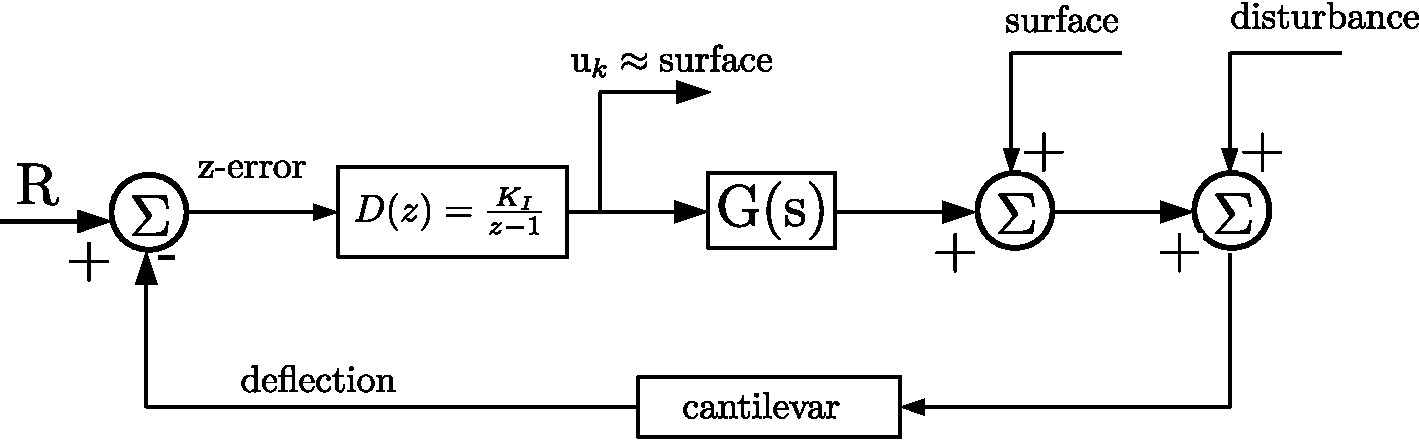
\includegraphics[width=0.7\textwidth]{plots_z_axis_improv/figures/AFM_loop.pdf}
  \caption{Block diagram of the $Z$-axis control loop, showing how disturbances from the sample surface and unwanted, external disturbances enter the control loop.}.
  \label{fig:zimprv:z_axis_bd}
\end{figure}

In general, the faster we scan, the larger bandwidth is needed in the $Z$-axis control loop. To see this, 
consider a (fictional) sample where the spatial frequency content is band-limited by frequency $f_{B_s}$ (i.e., the Fourier series describing the current scan line has a finite number of terms).
% Then the smallest wavelength in the current scan line is $\lambda_{B_s}=1/f_{B_s}$.
If we scan with speed $v$ then to the AFM probe, the surface, $s(t)$ appears in the time domain also band limited signal whose highest frequency component is
\begin{equation}
  f_{\textrm{surf}} = \frac{v}{\lambda}.
\end{equation}
Thus, as we scan faster, the surface presents as a higher frequency signal to the $Z$-axis control loop \cite{ando_highspeed_2008}.

We now show why we can take $u_Z$ to represent the sample surface. In general, $D(z)$ contains an integrator and $H_{ud}$ will be flat up to its roll off frequency $f_B$. Thus, if the frequency content of the surface $s$ is less than $f_B$, then from \eqref{eqn:hud}, $u \approx H_{ud}(1)s$. The upshot is that for any given control loop bandwidth, we can always\footnote{Assuming a sufficiently well behaved surface.} scan slowly enough so that most of the frequency content of the sample surface is less than $f_B$. If we wish to scan faster, we must increase $f_B$, or else the image will be distorted by the low-pass filtering nature of the control loop.

Now consider the situation when $d_{\text{ext}}\neq 0$. As illustrated in Fig.~\ref{fig:zimprv:z_axis_bd}, unwanted external disturbances enter the control loop at the same point as the sample surface.
This is because, e.g., from the perspective of the cantilever, the specimen vibrating vertically due a disturbance is indistinguishable from variations in the surface topology.
Thus, if the external disturbances are concentrated above some frequency $f_d$, then the $H_{ud}$ should roll-off before $f_d$ if we do not want those disturbances to corrupt the final image. This implies that we must artificially lower the scan speed to keep the specimen frequency content within the $H_{ud}$ bandwidth. Said another way, we must modulate the scan speed to induce a frequency separation between the external disturbances and the specimen. Thus, if we want to scan faster, we must extirpate as many external disturbances as possible.

% \begin{figure}[ht!]
%   \begin{subfigure}{.48\textwidth}
%     %                     L B R T  
%     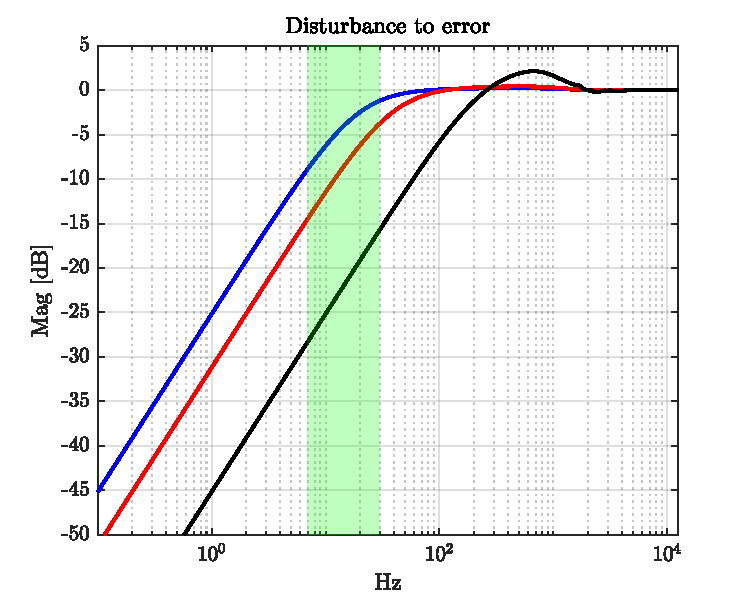
\includegraphics[trim=0 0 0 0, clip,width=1\textwidth]{plots_z_axis_improv/figures/Hde.pdf}
%     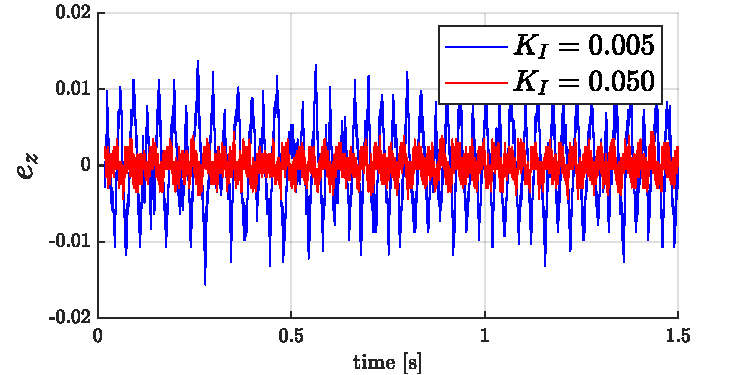
\includegraphics[trim=0 0 0 0, clip,width=1\textwidth]{plots_z_axis_improv/figures/ze_noise_example_Kis.pdf}
% \caption{Stuff }
% \label{fig:Hde}
% \end{subfigure}
% \hfill
%   \begin{subfigure}{.48\textwidth}
%     %                     L B R T  
%   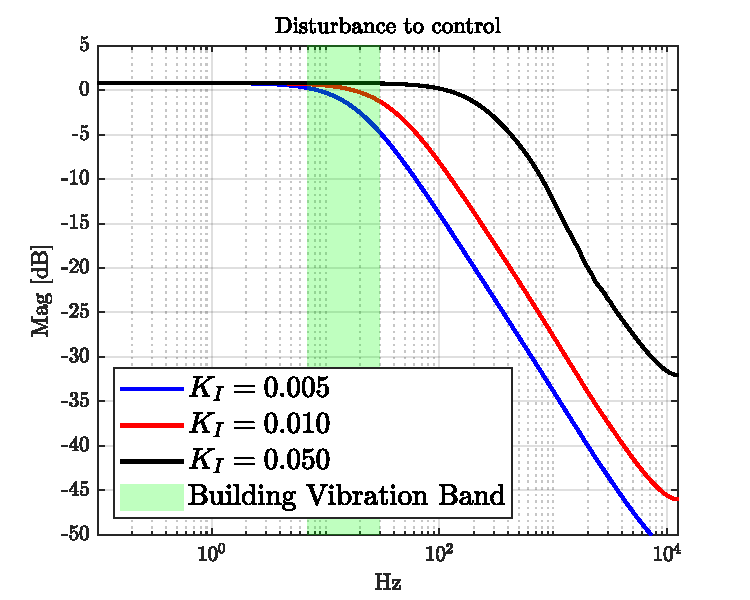
\includegraphics[trim=0 0 0 0, clip,width=1\textwidth]{plots_z_axis_improv/figures/Hdu.pdf}
%   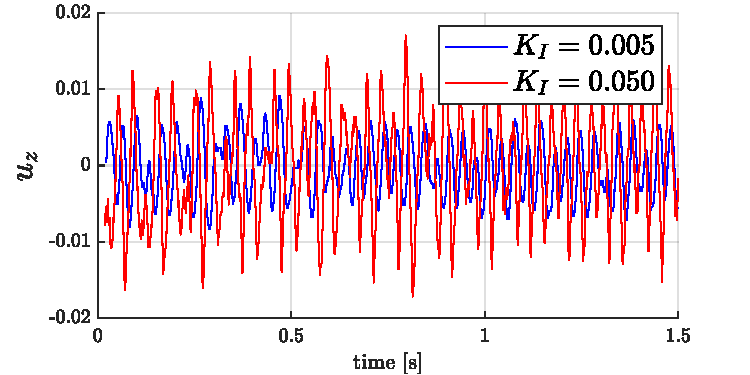
\includegraphics[trim=0 0 0 0, clip,width=1\textwidth]{plots_z_axis_improv/figures/uz_noise_example_Kis.pdf}
%   \caption{ }
%   \label{fig: Hdu}
% \end{subfigure}
% \caption{Control Loops.}
% \label{fig:z_improv:bode_loops}
% \end{figure}
% Figure~\ref{fig:z_improv:bode_loops} shows Bode diagrams for these two transfer functions for several values of $K_I$. On the one hand, we would like the bandwidth of $H_{ud}$ to be as high as possible because this will improve image quality. On the other hand, if we increase the bandwidth too much, we amplify the external noise sources, which are concentrated in the shaded green band. This means that we must keep the bandwidth artificially low to avoid corrupting our images with that noise. In turn, this means that the upper limit on the scan rate is set by the external disturbances, rather than limitations of the instrument mechanics. 

% The bottom row of plots in Fig.~\ref{fig:z_improv:bode_loops} shows the error and control signal in the time domain for two values of $K_I$. As one would expect, we do a better job rejecting disturbances with larger $K_I$. Unfortunately, we pay for this in the control signal. One might reasonably ask if this problem could be dealt with by leveraging the internal model principle to design a controller to specifically reject a sinusoid at 29 Hz. However, this will insert complex zeros on the imaginary axis which will ultimately produce artifacts in the image.

\section{Vibration Disturbances}
In this section, we characterize the external disturbances present in our experimental setup. 
To do this, we engage the cantilever with the sample surface, turn off all control loops, and measure the deflection signal. We then compute the power spectral density (PSD) of the deflection signal. This is shown in Fig.~\ref{fig:psd_xy_off} as the blue curve. This PSD is computed via Bartlett's method with 50 segments, each containing 32768 samples. 

The $XY$ stage is off in this experiment. Note the significant amount of energy present in the band stretching from about  7~Hz to 80~Hz, which is shaded in green. The bottom plot in Fig~\ref{fig:psd_xy_off} shows a portion of the time series used to compute the PSD. There the low frequency oscillations are clearly evident as well. Recall from Fig.~\ref{fig:G_mat_frf} that there are no oscillatory modes in the system dynamics between 7 to 80~Hz. Thus, we expect that energy to come largely from an external disturbance, as opposed to being due to white noise (say from the $Z$-axis power amplifier) becoming colored through one of $Z$-piezo modes. From the discussion in the previous section, if we don't want this energy in our images, we must severely de-rate the $Z$-axis control loop so that it rolls-off well before 10~Hz. 
\begin{figure}[t!]
  \includesvg[width=1\textwidth]{plots_z_axis_improv/figures/initial_dfl_psd_xyoff}
  \includesvg[width=1\textwidth]{plots_z_axis_improv/figures/initial_dfl_time_xyoff}
  \caption{The blue and red curves (left axis) are the PSD of the deflection signal with $XY$-stage off. The black curve is the FRF $H_{Z_d,u_Z}$.}
  \label{fig:psd_xy_off}
\end{figure}
Thus, we would like to eliminate these disturbances. The most likely culprit is building vibration, which may stem from, e.g., foot-traffic, the HVAC system, or other parts of the buildings mechanics. Of course, we are not alone in this problem and commercial solutions exist. Typical solutions range from purely passive systems \cite{keysight_vibration}, active vibration cancellation \cite{herzan}, and a combination of active cancellation and tuned mass-dampers \cite{newport}. These products are expensive. The simplest design is the purely passive system \cite{keysight_vibration}, which insert a mechanical low pass filter between the building and the AFM by suspending the AFM from bungee cords. 

The design is simple enough that it is straightforward construct a home-built alternative (shown in Fig.~\ref{fig:custom_isolator}) for about 70 USD. The idea is shown schematically in Fig.~\ref{fig:isolation_lpf}. The building's motion is represented as $p$ which is transfered to the AFM support (the mass $m$ through the spring and damper. The transfer function is given by
\begin{equation}
  x(s) = \frac{s\frac{\gamma}{m} + \frac{k}{m}}{s^2 + s\frac{\gamma}{m} + \frac{k}{m}}p(s).
  \label{eqn:vib_lpf}
\end{equation}

\begin{figure}[t!]
  \begin{minipage}[t]{.46\textwidth}
    \centering
    % L B R T
    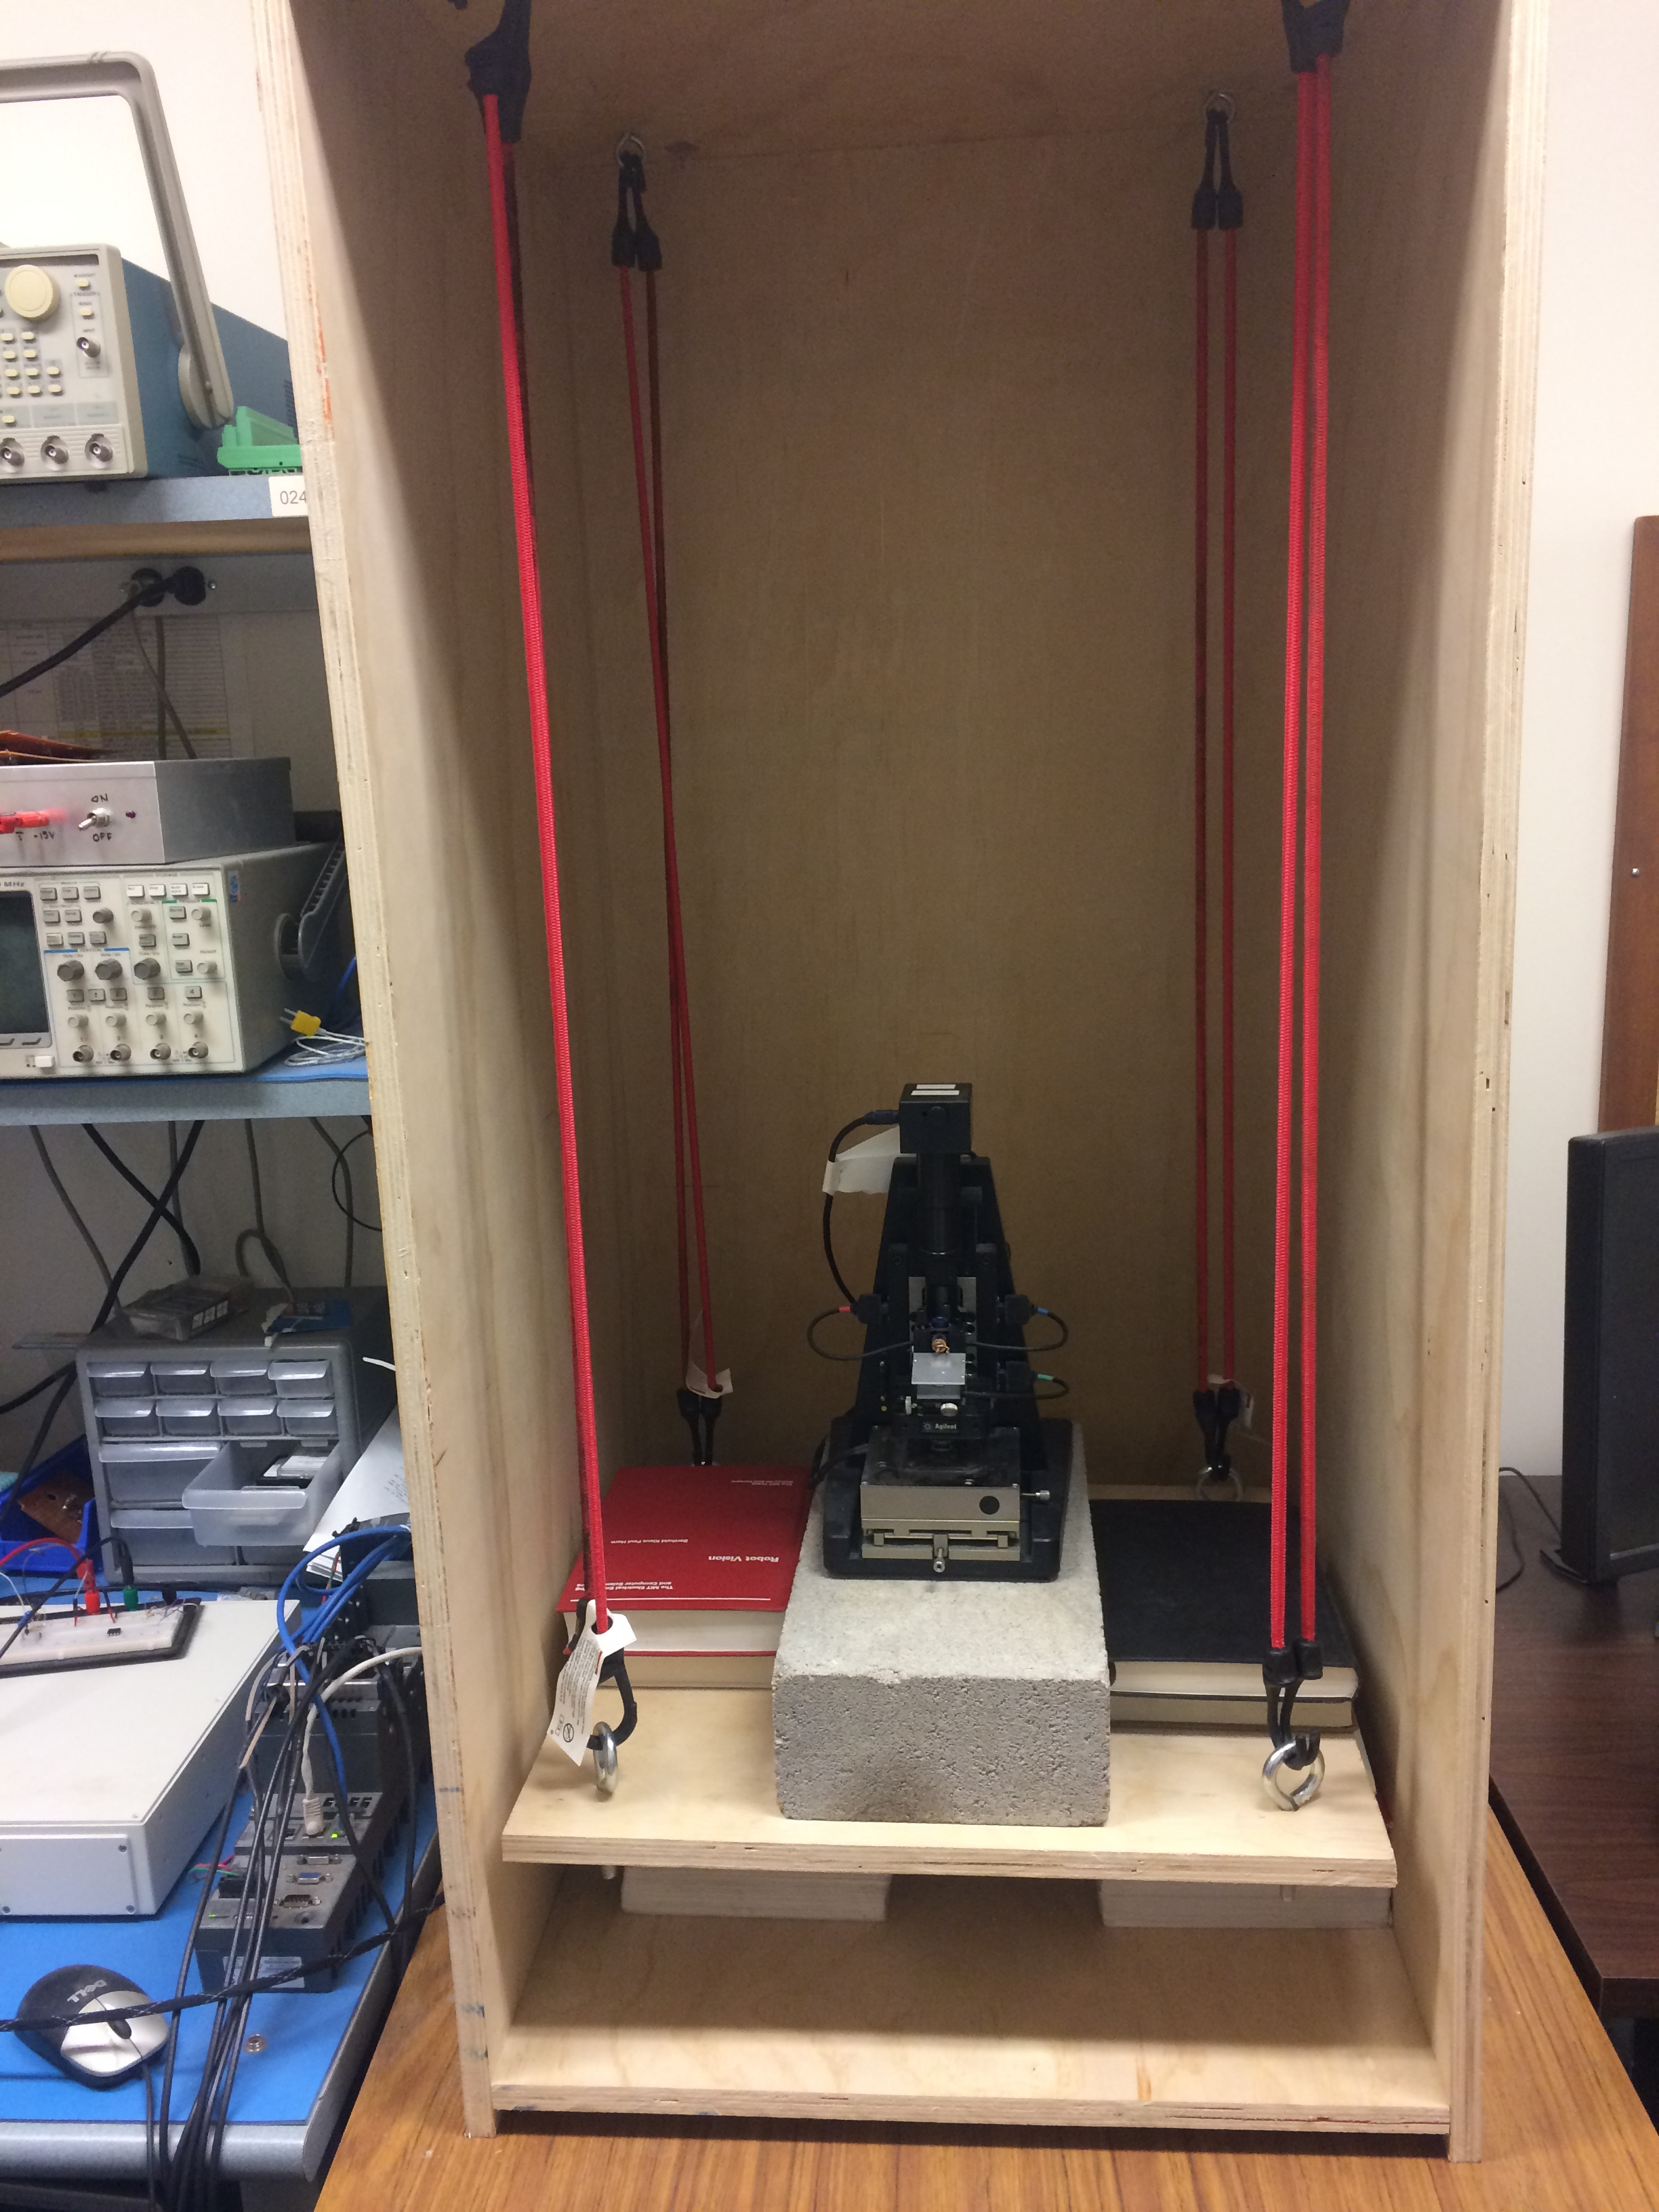
\includegraphics[trim=0 0 0 0,
    clip,width=0.7\textwidth]{plots_z_axis_improv/figures/my_isolator}
    \caption{Photograph of the home-build passive vibration isolator.}
    \label{fig:custom_isolator}
  \end{minipage}
\hfill
\begin{minipage}[t]{.46\textwidth}
  \centering
  % L B R T
  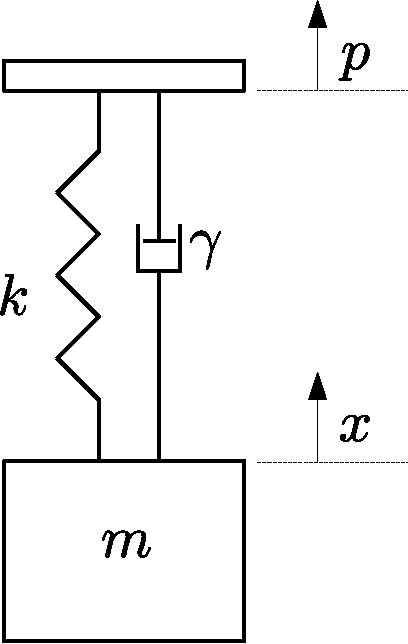
\includegraphics[trim=0 0 0 0,
  clip,width=0.5\textwidth]{plots_z_axis_improv/figures/mass-spring-damper.pdf}
  \caption{Schematic drawing of the bungee cord-based passive vibration
    isolation system.}
  \label{fig:isolation_lpf}
\end{minipage}
\end{figure}
To be effective, we need the cutoff frequency of this filter to be as small as possible, which means we need either $k$ small or $m$ large. It is difficult to control $k$, so we focus on making $m$ large, which is why there is a concrete block and books weighting the platform in Fig.~\ref{fig:custom_isolator}. The PSD which results after implementing this vibration mitigation scheme are shown in the top panel of Fig.~\ref{fig:psd_xy_off} as the red curve, which shows that the energy in the band from 10 to 80 Hz has been drastically attenuated. The reduction in low frequency vibration can also be seen in the red time series in bottom panel Fig.~\ref{fig:psd_xy_off}.

\section{Disturbances from Electrical Noise}
As noted, the above experiments were conducted in idealized circumstances: the $XY$-stage was powered off. We now move beyond that and conduct another similar set of experiments, this time with the $XY$-stage turned on. In the experiments to follow, the AFM is now always on the bungee system. The resulting PSD is shown as the blue curve in Fig.~\ref{fig:psd_xy_on_int}. In addition, the PSDs of $X$ and $Y$ axes are shown. 
Also plotted (against the right axis) in Fig.~\ref{fig:psd_xy_on_int} are FRFs of $G_{x,u_x}$ and $G_{y,u_y}$.

\begin{figure}[ht!]
  \begin{minipage}[t]{1\textwidth}
    \includesvg[width=1\textwidth]{plots_z_axis_improv/figures/initial_dfl_psd_xyon_intfan.svg}
    \caption{(left axis) PSDs of the $X$, $Y$, and $Z_d$ signals when the fan is powered by the C300. (right axis) FRFs of $G_{x,u_x}$ and $G_{y,u_y}$.}
    \label{fig:psd_xy_on_int}
  \end{minipage}
  \begin{minipage}[t]{1\textwidth}
    \includesvg[width=1\textwidth]{plots_z_axis_improv/figures/initial_dfl_psd_xyon_extfan.svg}
    \caption{PSDs of the $X$, $Y$, and $Z_d$ signals when the fan is powered by an external source.}
    \label{fig:psd_xy_on_ext}
  \end{minipage}
  \begin{minipage}[t]{1\textwidth}
    \includesvg[width=1\textwidth]{plots_z_axis_improv/figures/initial_dfl_time_xyon.svg}
    \caption{Time series of $Z_d$ when (blue) the fan is powered by the C300 and (orange) powered by an external source.}
    \label{fig:psd_xy_on_time}
  \end{minipage}
  % \caption{The blue and red curves (left axis) are the PSD of the deflection signal with $XY$-stage off. The black curve is the FRF $H_{Z,u_Z}$.}
  % \label{fig:psd_xy_on}
\end{figure}

There are two things to observe here. First, the resonances in the $XY$ stage now show up quite clearly in the $Z$-axis PSD. This is because the power amplifier output is not free of noise and thus, the $XY$-stage is now being driven, albeit, by a very small amount. This motion is coupled into the deflection signal. This can occur through both the sample tilt phenomenon discussed in Section~\ref{sec:non_param_frf} or through actual out-of-plane motion of the $XY$-stage. In either case, this is one reason low noise power amplifiers are desirable. 
Second, we have picked up a large spike in all three PSDs at 380~Hz and 760 Hz (the second harmonic of 380 Hz). Although there are sharp spike above in Fig.~\ref{fig:psd_xy_off}, those correspond to harmonics of 60~Hz. The spikes here at 380~Hz and 760~Hz are new features and not harmonics of 60~Hz.

\begin{figure}
  \begin{subfigure}{.48\textwidth}
    \centering
    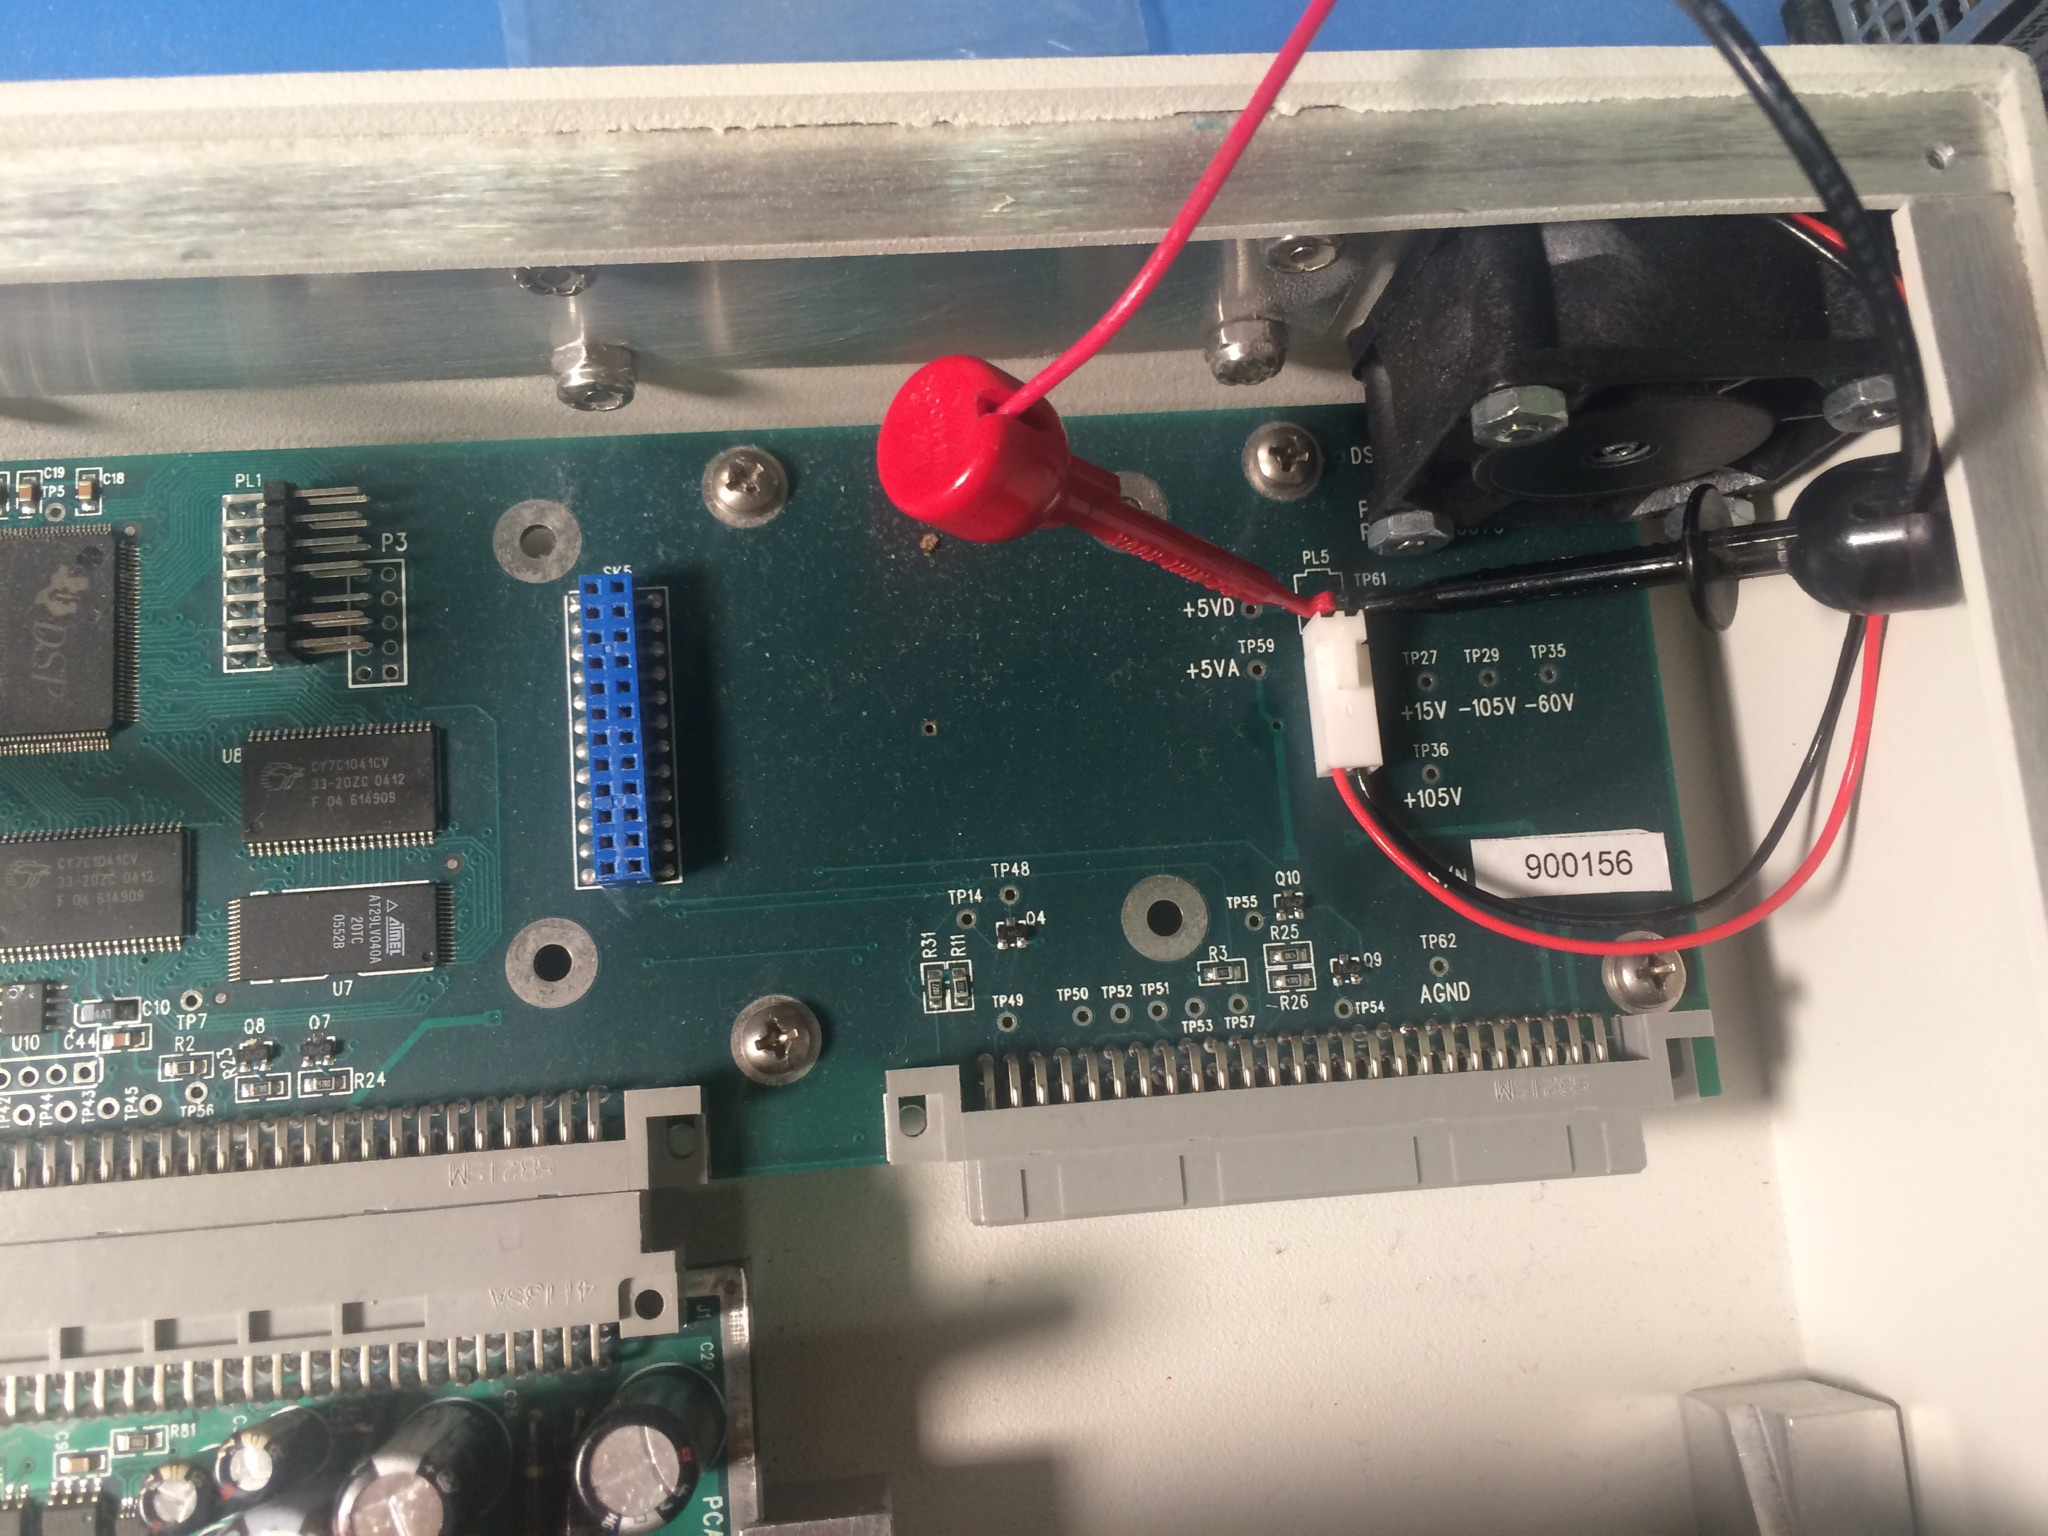
\includegraphics[width=0.8\textwidth]{plots_z_axis_improv/figures/c300_fan.jpg}
    \caption{ }
    \label{fig:c300_fan_pic}
  \end{subfigure}
  \begin{subfigure}{.48\textwidth}
    \centering
    \includesvg[width=1\textwidth]{plots_z_axis_improv/figures/fan_voltage.svg}
    \caption{ }
    \label{fig:c300_fan_voltage}
  \end{subfigure}
  \caption{(a) Photgraph of the C300 cooling fan. (b) Time-series of the fan voltage when the fan is plugged into the C300 circuit board (blue) and un-plugged (orange). In (b), the $x$-axis grids are spaced (1/380) seconds apart.}
  \label{fig: }
\end{figure}

Observe that the 380~Hz spike also occurs in the $X$ and $Y$ axis PSDs. We can trace this spike (mostly through luck) to the cooling fan inside the C300. If we unplug the fan from the circuit board (see Fig.~\ref{fig:c300_fan_pic}) and run it from an external power source, we get the orange curves in Fig.~\ref{fig:psd_xy_on_ext}: the spikes at 380~Hz and 760~Hz are now completely gone from all three PSDs. Fig.~\ref{fig:psd_xy_on_time} compares $Z_d$ time-series data for two scenarios, which shows a significant reduction in the overall amplitude.

The time-series in Fig.~\ref{fig:c300_fan_voltage} shows the fan voltage supply when the fan is plugged in (blue) and un-plugged (red). The period of oscillation in the blue curve is approximately 380~Hz. Evidently, the power source driving the fan inside the C300 is insufficiently decoupled from the voltage driving piezo stage. Thus, the XY stage oscillates at 380~Hz and this is coupled into the deflection via sample tilt.

\subsubsection{Results}\label{sec:bungee_results}
\begin{figure}[t!]
  \begin{subfigure}{.48\textwidth}
    %                     L B R T  
    \includesvg[width=1\textwidth]{plots_z_axis_improv/figures/raster_nobungee.svg}
    \caption{}
    \label{fig:raster_no_bung}
  \end{subfigure}
  \begin{subfigure}{.48\textwidth}
    %                     L B R T  
    \includesvg[width=1\textwidth]{plots_z_axis_improv/figures/raster_bungee.svg}
    \caption{ }
    \label{fig:raster_with_bung}
  \end{subfigure}
  \caption{Raster scan results over a 5 micron square area of the CS20-NG sample grating. The two bottom panels show a cross section of the rows of pixels indicated by color in the top two panels. (left) Before disturbance mitigation and (right) with both vibration isolation and isolating the C300 fan's electrical supply.}
  \label{fig:raster_dist_results}
\end{figure}
Fig.~\ref{fig:raster_dist_results} shows two raster scans of the CS20-NG sample grating. The scans were taken over a 5 micron square area at a scan rate of 1~Hz. The scan shown in Fig.~\ref{fig:raster_no_bung} was taken with the standard setup: i.e., the AFM is positioned on a table and the C300 fan is driven from the internal power supply. The scan shown in Fig.~\ref{fig:raster_with_bung} was taken with both mitigations, that is, using the bungee-based vibration isolator and with an external power source driving the C300 fan. Both scans were taken back to back with the same tip and the scan in \ref{fig:raster_no_bung} was taken first.

The bottom two panels show a cross section of the pixels indicated by the red and blue lines in the images. Of particular note are the red curves, which show the performance over the flat areas of the grating. The improvement seen in the right panel is drastic compared to the native instrument.

\subsubsection{Disadvantages}
The bungee cord vibration isolation method is not without disadvantages. The most notable problem is we cannot control the damping. From \eqref{eqn:vib_lpf}, the system damping $\zeta$ is given by
\begin{equation}
  \zeta = \frac{\gamma}{\sqrt{km}}.
\end{equation}
Thus, by increasing $m$, we decrease the damping, which means that near the natural frequency of our low pass filter, we have introduced a resonance with little damping. This will amplify vibrations whose frequency is near $\sqrt{k/m}$. However, these will be very low frequency oscillations, and if we follow the common practice of de-trending each scan line, do not seem to present significant difficulties.

% In Fig.~\ref{fig:raster_dist_results}, we de-trended each scan line. While this is a common post-processing technique in AFM, it introduces some artifacts and hides others. For example, in Fig.~\ref{fig:raster_dist_results}, it would appear that the area between the holes (in the $X$-directions) is higher than the flat areas between the holes in the $Y$-direction. We do not expect this to be the case from the specification of the CS20-NG. We may alternatively, de-trend the entire plane. An example of this is shown in Fig.~\ref{fig:undulation}. 

% \begin{figure}[t!]
%   \includesvg[width=0.5\textwidth]{plots_z_axis_improv/figures/raster_no_bungee_mesh}
%   \includesvg[width=0.5\textwidth]{plots_z_axis_improv/figures/raster_bungee_mesh}
%   \caption{}
%   \label{fig:undulation}
% \end{figure}

% What we see is that, indeed, the bungee has system has eliminated most of the local noise (i.e., along the $X$-direction). Arguably, the oscillations in the $Y$-direction, which would correspond to frequency content of less than a tenth of a Hz (the scans takes approximately 5 minutes), have become worse.

\section{Z-axis Control Design}\label{sec:zaxis_cs_control}
In Section~\ref{sec:zaxis-dist}, we eliminated or reduced many of the disturbances impinging on the $Z$-axis. 
This puts us in a position to increase the bandwidth without introducing building dynamics into our images.
The main challenge to increasing the $Z$-axis bandwidth is the bending mode resonance at 215 Hz, which can be seen in the FRF from $u_Z$ to $Z_{d}$ in Fig.~\ref{fig:z_control} (blue curve). We address this by inverting the complex pole-zero pair at 215 Hz. There are multiple advantages to this method: first, an inverse compensator still makes sense as a feedforward, open-loop compensator if the feedback path is broken. This,  situation can and does occur during parts of the CS cycle. Second, as we discuss further below, the inverse compensator requires no tuning as it is defined only by a fit to the measured FRF and this can be almost completely automated. 

\begin{figure}[b!]
  \centering
  \includesvg[scale=0.9]{plots-afm-cs-final/figures/z_control_design.svg}
  \caption{}
  \label{fig:z_control}
\end{figure}
The entire $Z$-axis controller consists of a PI controller, $D_I(z)$ cascaded with the resonance inversion, $D^{-1}(z)$. The inclusion of $D^{-1}$ allows us to substantially increase the PI gain and achieve a closed-loop bandwidth of about 480 Hz. This is the black curve in Fig.~\ref{fig:z_control}.
For comparison, the red curve in Fig.~\ref{fig:z_control} shows the closed-loop FRF without the inverse compensator, which experiments indicate is unstable.

One challenge to this approach is the system gain and resonance at 215~Hz changes not only day-to-day but also (and especially) when changing cantilevers. This is illustrated in Fig.~\ref{fig:z_evolution}, which shows the FRF near the mode for two three different cantilevers. Two are of the same make and model.

One cause for such different gains is variation in the length of the cantilever (and possibly how the laser was adjusted). This is illustrated in Fig.~\ref{fig:z_axis_gain}. Here, we consider a cantilever with length $h$ that rests on the surface of some specimen with a nominal angle of $\theta$. In this drawing, the laser is perpendicular to the sample surface. Given a vertical perturbation $\Delta z$, we have that
\begin{equation}
  \Delta \alpha \approx \frac{d}{h} \Delta z,
\end{equation}
where $d$ is the distance from the cantilever to the detector and $\Delta \alpha$ is the change in position of the incident laser spot on the detector. Thus, given the same change in the vertical position, we will see a larger change in the deflection signal for a shorter cantilever. In other words, a short cantilever will exhibit a larger DC-gain in the $G_{u_Z,Z_d}$ transfer function. 
\begin{figure}
    \begin{minipage}[t]{.46\textwidth}
    %                     L B R T  
    \includesvg[width=1\textwidth]{plots-afm-cs-final/figures/z_cant_evolution.svg}
    \caption{FRFs of three different cantilevers, showing substantial differences in the DC-gain and smaller, but still significant differences the frequency of the modes.}
  \label{fig:z_evolution}
\end{minipage}
\hfill
  \begin{minipage}[t]{.46\textwidth}
    % L B R T  
  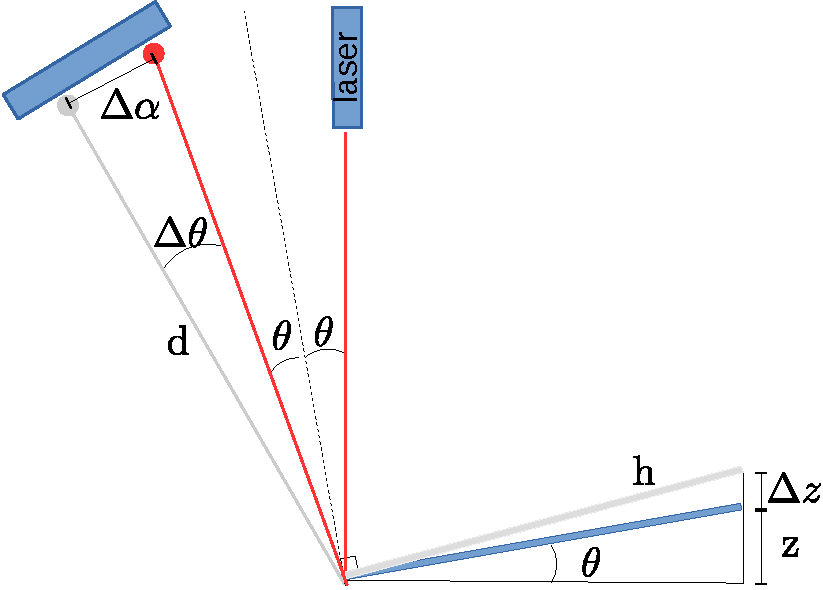
\includegraphics[width=1\textwidth]{plots-afm-cs-final/figures/z_axis_gain_schematic-crop.pdf}
    \caption{Schematic drawing of how the length of the cantilever affects the $z$-axis gain.}
    \label{fig:z_axis_gain}
  \end{minipage}
\end{figure}

Fig.~\ref{fig:z_evolution} shows the frequency response of $G_{u_Z,Z_d}$ near the bending mode for three different cantilevers. Cantilevers (A) and (B) are both AppNano SICON cantilevers and have a nominal length of 450 microns. Cantilever (C) is an NCLR and has a nominal length of 225 microns. Interestingly, the SICON cantilevers show substantial variation. Unfortunately, the manufacture does not provide a tolerance on the nominal length, so it is difficult to tease out whether that variation is due to manufacturing variability or other factors not explained by this analysis.

Notably, the frequency of the pole and zero do appear to shift and our inversion scheme is not robust to this.
To deal with this, I have built a (mostly) automated system ID routine into the imaging software. This routine is a specialized version of the techniques described previously in Chapter~\ref{chap:modeling}. First, it obtains an FRF of the bending mode over a frequency range spanning 180~Hz to 240~Hz (the same set of points as in Fig.~\ref{fig:z_evolution}). The input and output sinusoids are demodulated in quasi-realtime as they come off the FPGA. Once this is complete, a 2-pole, 2-zero transfer function model of the form
\begin{equation*}
  \hat{D}(z) = k \frac{z^2 + b_1z + b_o}{z^2 + a_1z + a_o}
\end{equation*}
is fit to the FRF, using the same optimization scheme as \eqref{eqn:logfit}.
This is done inside the LabView VI by calling a custom DLL, which leverages CMPFIT~\cite{cmpfit,markwardt_mpfit_2009}, a Levenberg-Marquardt~\cite{more_levenberg_1978} routine written in C.
To promote a stable fit, the optimization enforces the necessary conditions that
\begin{align*}
  |a_1| &< 2, \quad  |a_o| < 1\\
  |b_1| &< 2, \quad  |b_o| < 1.
\end{align*}
The routine then checks that both the poles and zeros are indeed stabile, saves the data to a JSON file and passes the transfer function parameters into the imaging portion of the application which finally uploads the parameters into the FPGA imaging bitfile. Optionally, one can by-pass this step and simply load the previously saved JSON file.

One of the benefits of this approach is that the DC-gain of the transfer function $G_{u_Z,Z_d}$  becomes (approximately) normalized to unity, which makes re-tuning the control system after changing tips far easier to non-existent. The benefit to automating the process is that it drastically reduces the friction required to obtain an up-to-date compensator, which means that an up-to-date compensator is more likely to be used~\cite{abramovitch_25years_2015}.


Fig.~\ref{fig:afm_bd_dinv} shows a block diagram if the $Z$-axis control loop. We point out a small change from Chapter~\ref{chap:cs_init}: the addition of $D^{-1}(z)$ changes the correct signal to use to represent the sample surface. If we take the output of the entire compensator, $u_Z=D_ID^{-1}e_z$, then we will get a lot of wiggles in the resulting signal. Rather, we need to take only the output of the integrator to represent the surface. 
\begin{figure}
  \centering
  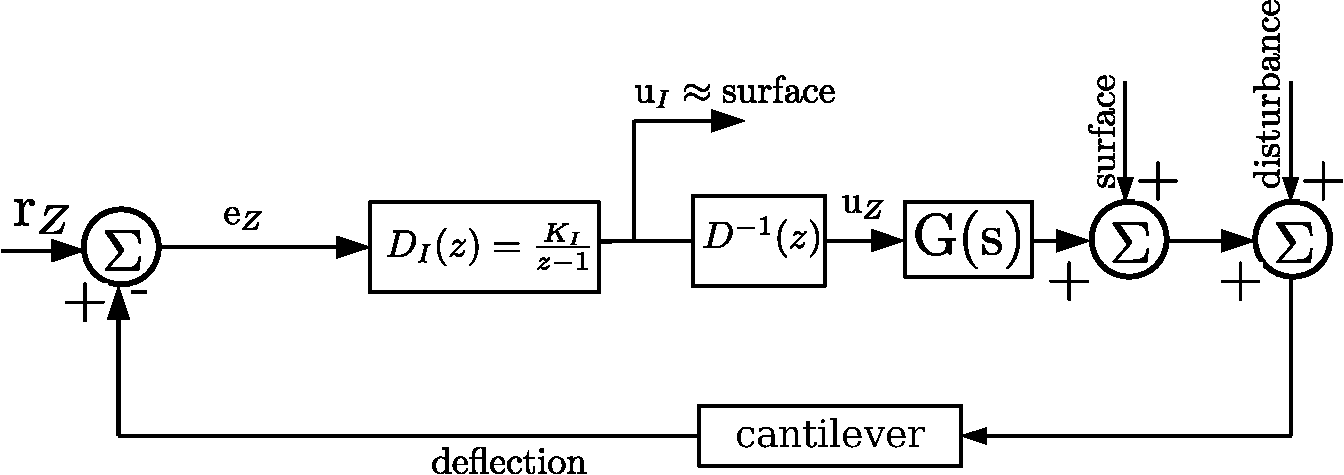
\includegraphics[scale=0.5]{plots-afm-cs-final/figures/AFM_loop_Dinv-crop.pdf}
  \caption{Block diagram of the $Z$-axis control loop with the inverse compensator. }
  \label{fig:afm_bd_dinv}
\end{figure}


It should be noted that this control is sufficient to eliminate the limit-cycle behavior described in Section~\ref{sec:aproachspeed}: we have done many CS scans across many variations of the CS-state machine using this control scheme and the limit cycle has not appeared. The resulting bandwidth of about 480~Hz is substantially higher than what we had in Chapter~\ref{chap:cs_init}. Unfortunately, although I recorded the Integral gain used in the initial implementation described in Chapter~\ref{chap:cs_init}, I do not know what the system gain was for that specific cantilever, so it is not possible to make that comparison quantitatively. Based on the improved scan rates achieved in the next chapter,  (see e.g., Fig.~\ref{fig:pixel_rows}), I would estimate the improvement to be between 5 and 10 times.


% \subsubsection{Caveats to Inversion}
% \textbf{ACTUALLY: maybe this is really just larger oscillations from a larger move size??}

% It seems that inversion favors raster scanning over CS.

% The issue, I believe and need to demonstrate more fully, is that the nature of the resonance can shift depending on the setpoint and especially the input magnitude (for sinusoidal inputs). During CS, we ask the system to operate over a wider range, and thus these non-linearties play a larger role. This is evident in Fig.~\ref{fig:dinv_CS_decay}, where we have connected multiple $\mu$-paths together. What we see is oscillations after the engagement and in the first scan, but which decay after the first hole. Thus, the inversion is more than capable when operating in the limited range around which it was identified, but performance degrades during the approach, which is away from the point at which it was identified.


% \begin{figure}
%   \centering
%   \includesvg[scale=0.8]{plots-afm-cs-final/figures/dinv_CS_cycle_decay.svg}
%   \caption{}
%   \label{fig:dinv_CS_decay}
% \end{figure}

%%% Local Variables:
%%% mode: latex
%%% TeX-master: "thesis_main"
%%% End:
